\section{\textLR{SwinTrack\cite{swinTrack}}\label{section:swintrack}}
الفكرة الأساسية من البحث هي تعديل ملاحق
\textLR{SwinTrack}
بإدخال المعلومات الزمانية، وذلك بالاستفادة من التعديل المستخدم في ملاحق 
\textLR{STARK}
\ref{section:stark}. 
لذلك سنشرح في هذه الفقرة خوارزمية 
\textLR{SwinTrack}
بشيء من التفصيل، كونها النموذج الأساسي في بحثنا.
\newline
هذا الملاحق يعتمد كلياً على توابع الانتباه لاستخلاص ودمج السمات، إذ أنه يستخدم محول
\textLR{Swin\cite{swintransformer}}
كـ
\textLR{backbone}
لاستخلاص السمات، وبذلك فهو يختلف عن الملاحقات السابقة التي تستخدم المحول كجزء من بنيتها، وتستفيد من شبكات
\textLR{CNN}
%كشبكة
%\textLR{ResNet\cite{ResNet}}
%وشبكة
%\textLR{AlexNet\cite{alexnet}}
لاستخلاص سمات الصور، وذلك كما في خوارزميات الملاحقة
\textLR{Transformer Tracking\cite{transformertracker}}
و
\textLR{STARK\cite{Stark}}.
أما بالنسبة لخوارزمية الملاحقة 
\textLR{SwinTrack}
فهي تستخدم بنية  مرمز- مفكك ترميز
%\textLR{encoder-decoder}
لدمج السمات والتي تعتمد على توابع الانتباه كما في المحول الأصلي
\textLR{\cite{Vaswani17}}. 

\begin{figure}[!h]
	\centerline{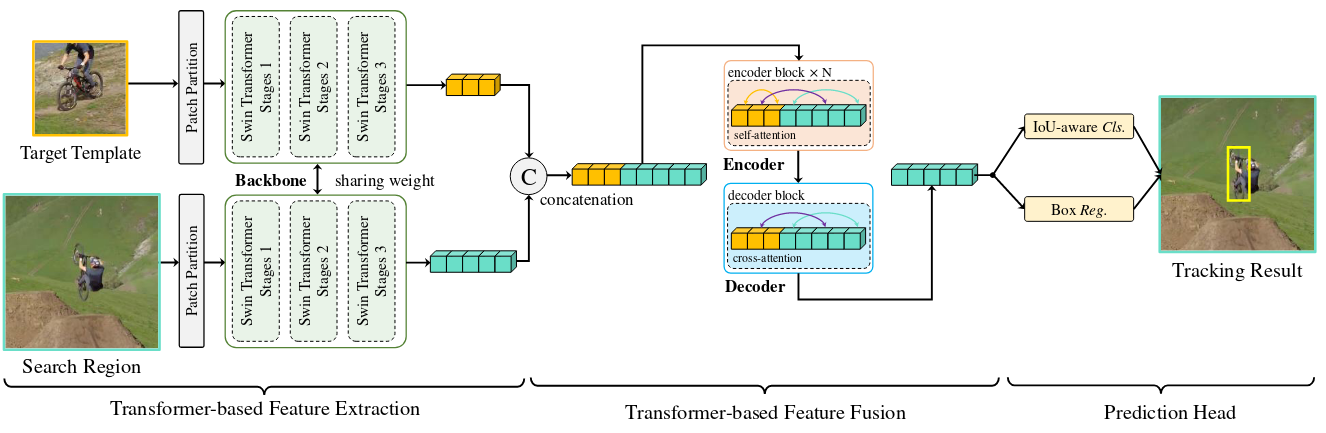
\includegraphics[width=\textwidth]{images/swinTrack}}
	\caption{
		\textRL{بنية الملاحق}
		\textLR{SwinTrack}
		\textLR{\cite{swinTrack}}}
	\label{fig:swintrack}	
\end{figure}
يوضح الشكل 
\ref{fig:swintrack}
مراحل خوارزمية 
\textLR{SwinTrack}،
وهي بشكل أساسي تتكون من ثلاث مراحل، الأولى لاستخلاص السمات، والثانية لدمجها، والثالثة لتحديد مكان وأبعاد الغرض، وسنشرح في الجزء التالي كل مرحلة من هذه المراحل.
\subsection{المرحلة الأولى - استخلاص السمات}
تستخدم هذه الخوارزمية  المراحل الثالث الأولى من محول
\textLR{Swin}
كـ
\textLR{backbone}.
وبمقارنة محول
\textLR{Swin}
بشبكات
\textLR{CNN}
الأخرى
\textLR{\cite{alexnet}\cite{ResNet}}،
 فإن محول
\textLR{Swin}
قادر على إعطاء تمثيل للسمات بشكل أفضل
\textLR{\cite{swintransformer}}.
يوضح الشكل 
\ref{fig:swintrack}
مداخل نموذج الملاحقة 
\textLR{SwinTrack}،
حيث له دخلان الأول هو صورة الـ 
\textLR{template}
الإبتدائي،
والثاني هو نافذة البحث.
\newline
تم تجريب ثلاث نسخ من محول 
\textLR{Swin}
كـ
\textLR{backbone}.
وفيما يلي أبعاد كل نموذج بحسب الـ
\textLR{backbone}
المستخدمة:

\selectlanguage{english}
	\begin{itemize}
		\item SwinTrack-T
		\newline
		Backbone: Swin Transformer-Tiny\cite{swintransformer}
		\newline
		Template size: [112 x 112]; Search region size [224 x 224]; C = 384; N=4
		
		\item SwinTrack-B
		\newline
		Backbone: Swin Transformer-Base\cite{swintransformer}
		\newline
		Template size: [112 x 112]; Search region size [224 x 224]; C = 512; N=8
		
		\item SwinTrack-B-384
		\newline
		Backbone: Swin Transformer-Base\cite{swintransformer}
		\newline
		Template size: [192 x 192]; Search region size [384 x 384]; C = 512; N=8
	\end{itemize}
\selectlanguage{arabic}
حيث $C$ هو بعد النموذج و
$s=16$
هو 
\textLR{stride}
الشبكة،
\textRL{
		و
		$N$
		عدد كتل المرمز
}.
\newline
\subsection{المرحلة الثانية - دمج السمات بالاعتماد على المحول}
يتم سَلسَلة سمات الـ
\textLR{template}
وسمات نافذة البحث ضمن تمثيل موحد $U$ يشكل دخلاً للمرمز.
وكما في المحول الأصلي فإن المرمز يتكون من 
توابع انتباه ذاتي متعددة الرؤوس 
\textLR{MSA}،
مع شبكة عصبونية 
\textLR{FFN}
تتكون من طبقتين مع تابع تفعيل
\textLR{GELU}
\textLR{Gaussian Error Linear Unit}،
مع وجود تنظيم خطي 
\textLR{Linear Normalization}
قبل كل كتلة
\textLR{\textLR{FFN} + MSA}،
و 
\textLR{Residual connection}
 بعد كل كتلة 
\textLR{\textLR{FFN} + MSA}،
وذلك بحسب المعادلات 
\ref{eq:swinencoder}
\begin{equation} \label{eq:swinencoder}
\begin{split}
 &U^1 = Concat(z^1,x^1)\\
 &...\\
 &U^{l^\prime} = U^l + MSA(LN(U^\prime))\\
 &U^{l+1} = U^{l^\prime} + FFN(LN(U^{l^\prime}))\\
 &...\\
 &z^L,x^L = Deconcat(U^L)
\end{split}
\end{equation}


حيث $l$ هي رقم الطبقة، $L$ عدد طبقات المرمز.
كما نرى في آخر معادلة وبحسب الشكل
\ref{fig:swintrack}
فإنه يتم إعادة فصل 
\textLR{deconcatenate}
خرج المرمز وتقسيمه إلى سمات الـ
\textLR{template}
وسمات نافذة البحث.
\newline
يتبع نموذج المحول الأصلي
\textLR{\cite{Vaswani17}}
الطريقة التقليدية في
دمج ومعالجة السمات الآتية من مصادر مختلفة (المصدران في حالتنا هما
\textLR{template}،
ونافذة البحث)، وذلك بحساب الانتباه الذاتي لكل مصدر أي لصورة ال
\textLR{template}
ولصورة نافذة البحث بشكل مستقل، ومن ثم دمج هذه السمات عن طريق 
\textLR{cross-attention}.
هذه الطريقة تدعى بـ
$"$
دمج السمات بالاعتماد على الانتباه التقاطعي
$"$.
%\textRL{بالاعتماد}
% على
%\textLR{cross-attention}$"$.
\newline
أما الطريقة المتبعة في ملاحق
\textLR{Swin}
هي بدمج السمات في دخل المرمز ومعالجتها كسلسلة واحدة، وتسمى بـ
$"$
دمج السمات بالاعتماد على السَلسَلة
\textLR{concatenation-based fusion}
$"$.
وبمقارنة هذه الطريقة بالطريقة السابقة فإنها تخفض التعقيد الحسابي وذلك بانقاص عدد أوزان النموذج، 
\textRL{وبالتالي فهي مناسبة أكثر لتطبيقات الزمن الحقيقي}
\newline
تابع الانتباه هو التابع المستخدم في المحول الأصلي
\textLR{\cite{Vaswani17}}،
إذ لا حاجة لاستخدام تابع انتباه
\textLR{Swin}،
لأن الفرق في التعقيد الحسابي بين التابعين بسيط في حالة دخل صغير الأبعاد، والدخل هنا هو أشعة السمات.
\newline
ترميز الموقع
\textLR{Positional Encoding PE}:
لمساعدة النموذج على تمييز مصادر وأماكن السمات التي تتم معالجتها لابد من إضافة ترميز مكاني إلى السمات، والنوع المستخدم في 
\textLR{SwinTrack}
هو 
\textLR{Untied Positional Encoding\cite{untiedPE}}.
\newline
أما بالنسبة لدخل  مفكك الترميز
 فهو عبارة عن السمات الخارجة من المرمز، وخرجه هو خريطة السمات المعدلة لنافذة البحث
$ x \in \Re^{\frac{H_x}{s} \mathsf{x} \frac{W_x}{s} \mathsf{x} C}$.
تتبع العمليات الحسابية ضمن مفكك الترميز
المعادلات 
\ref{eq2}:
\begin{equation} \label{eq2}
\begin{split}
&U^D = Concat(z^l,x^l)\\
&x^{L^\prime} = x^L + MCA(LN(x^L),LN(U^D))\\
&x = x^{L^\prime} + FFN(LN(x^{L^\prime})).\\
\end{split}
\end{equation}
يحسب تابع الانتباه التقاطعي متعدد الرؤوس
\textLR{MCA}
بين
$x^L$
 خريطة سمات نافذة البحث بعد فك السلسلة، وبين 
$U^D$
%\textLR{Ud}
خرج المرمز والذي يعبر عن سمات كل من الـ
\textLR{template}
ونافذة البحث.
\subsection{المرحلة الثالثة - شبكتي التصنيف وال 
\textLR{regression}
	: }
الخرج النهائي لمفكك الترميز
هو سمات نافذة البحث
$x \in \Re^{\frac{H_x}{s} \mathsf{x} \frac{W_x}{s} \mathsf{x} C}$،
هذه السمات بحاجة إلى معالجة لتحديد موقع الغرض بالنسبة لنافذة البحث.
\newline
يتم استخدام طريقتي التصنيف والـ  
\textLR{regression}
  بشكل منفصل لتحديد موقع الغرض والمستطيل المحيط به.
كل من الكتلتين عبارة عن شبكة عصبونية
\textLR{MLP}
تتكون من ثلاث طبقات، ودخل كل من الشبكتين هو خرج مفكك الترميز.
\newline
الكتلة الأولى هدفها التصنيف ضمن صنفين هما الهدف والخلفية، وخرجها هو خريطة استجابة التصنيف
\textLR{classification response map}
$r_{cls} \in \Re^{(H_x \mathsf{x} W_x) \mathsf{x} 1}$،
بحيث تكون قيمة كل عنصر من عناصر المصفوفة  ضمن المجال
$[0,1]$،
وهذه القيمة تعبر عن احتمالية وجود الغرض في هذا الموقع.
\newline
أما الكتلة الثانية وهي الـ 
\textLR{regression}،
فغايتها التنبؤ بالمستطيل المحيط، وخرجها 
$r_{reg} \in \Re^{(H_x \mathsf{x} W_x) \mathsf{x} 4}$،
كل عنصر من عناصر الخرج يعبر عن إحداثيات الزاوية العليا اليسارية و الزاوية السفلى اليمينية  للمستطيل المحيط.
\newline
%يتم معالجة خرج الشبكتين لتحديد موقع الغرض، فمثلا تم افتراض أن حركة الهدف انسيابية فيتم استخدام 
%\textLR{Hanning penalty}
%للحد من الحركات الكبيرة.
%وفي النهاية
لتحديد موقع الغرض يتم اختيار المستطيل المقابل لأعلى استجابة تصنيف.
وكما لاحظنا من بنية الملاحق فإنه يعتمد بشكل كلي على مظهر الغرض في الإطار الأول للملاحقة دون الأخذ بعين الاعتبار تغيرات شكل الغرض. 
%\textLR{AdamW\cite{AdamW}}
\begin{table}[!h]
	\centering
	\begin{tabular}{c c c c c c c} 
		\hline
		\textLR{Tracker} & $mAO$\% & $mSR_{50\%}$ & $mSR_{75\%}$ &\textLR{Speed($fps$)}&\textLR{FLOPS(G)}&\textLR{Params(M)}\\ [0.5ex] 
		\hline\hline
		\textLR{STARK-S50} &$67.2$&$76.1$&$61.2$&$41.8$&$10.5$&$32.3$\\
		\textLR{STARK-ST50} & $68.0$ & $77.7$ & $62.3$&$41.8$&$10.9$&$32.5$\\ 
		\textLR{STARK-ST101} &$68.8$ & $78.1$ & $64.1$&$31.7$&$18.5$&$42.4$\\
		\hline
		\textLR{SwinTrack-T} & $69.0$ & $78.1$ & $62.1$&$98$&&$23$ \\
		\textLR{SwinTrack-B} & $69.4$ & $78.0$ & $64.3$&$52$&&$91$ \\
		\textLR{SwinTrack-B} &&&&$45$&&$91$\\[1ex] 
		\hline
	\end{tabular}
	\caption{
		\textRL{نتائج خوارزميتي}
		\textLR{SwinTrack,STARK}
		\textRL{من أجل معطيات التدريب}
		\textLR{GOT-10k\cite{got10k}}}
	\label{table:two_tracker_got10k_results}
\end{table}
\newline
%\begin{table}[!h]
%	\centering
%	\begin{tabular}{c c c c c c c} 
%		\hline
%		\textLR{Tracker} & \textLR{AUC}\% & \textLR{Normalized Precision} & \textLR{Precision}&\textLR{Year}\\ [0.5ex] 
%		\hline\hline
%		\textLR{SwinTrack-B-384} &$70.2$&$78.4$&$75.3$&$2021$\\
%		\textLR{STARK} & $67.1$ & $77.0$ &&$2021$\\ 
%		\textLR{TransT} &$64.9$ & $73.8$ & $69.0$&$2021$\\
%		\textLR{TrTr} & $55.1$ &&&$2021$&\\[1ex] 
%		\hline
%	\end{tabular}
%	\caption{
%		\textRL{نتائج خوارزميتي}
%		\textLR{SwinTrack,STARK}
%		\textRL{من أجل معطيات التدريب}
%		\textLR{GOT-10k\cite{got10k}}}
%	\label{table:many_tracker_got10k_results}
%\end{table}

 يوضج الجدول
 \ref{table:two_tracker_got10k_results}
نتائج اختبار خوارزميتي 
\textLR{STRAK\cite{Stark}}
و
\textLR{SwinTrack\cite{swinTrack}}
من أجل مجموعة المعطيات 
\textLR{GOT-10k\cite{got10k}}.
نلاحظ تفوق خوازمية
\textLR{SwinTrack}
في الأداء والسرعة على خوارزمية
\textLR{STARK}.
ونلاحظ أن النسخة
\textLR{SwinTrack-T}
أسرع بمرتين تقريبا من النسخ الأخرى، وهذا ما شجعنا على استخدامها كنموذج أساسي في بحثنا، وتطوير هذه الخوارزمية للحصول على أداء أفضل مع سرعة ملاحقة عالية.
\iffalse
\begin{table}[H]
	\centering
	\begin{tabular}{||p{2.cm}||p{2.cm}||p{2.cm}||p{2.cm}||}
		\hline
		Tracker 	& SwinTrack-Tiny-t4 &\\
		\hline
		SS   		& 79.7 \\
		PS 			& 71.6 \\ 
		NPS 		& 90.1 \\ 
		AO 			& 81.2 \\ 
		SR$_{50\%}$ & 91.1 \\ 
		SR$_{75\%}$ & 79.0 \\
		FPS 		& 66.6\\
		HW 			& NVIDIA GeForce RTX 3060 Laptop GPU\\
		\hline
	\end{tabular}
	\caption{SS : Success Score ,PS : Precision Score , NPS : Normalized Precision Score.
	\newline
	validation}
	\label{table:1}
\end{table}

\label{table:2}
\fi

%
%%report
%\begin{table}[!h]
%	\centering
%	\begin{tabular}{c c c c c c c} 
%		\hline
%		\textLR{Tracker} & $mAO$\% & $mSR_{50\%}$ & $mSR_{75\%}$ &\textLR{Speed($fps$)}&\textLR{FLOPS(G)}&\textLR{Params(M)}\\ [0.5ex] 
%		\hline\hline
%		\textLR{STARK-S50} &$67.2$&$76.1$&$61.2$&$41.8$&$10.5$&$32.3$\\
%		\textLR{STARK-ST50} & $68.0$ & $77.7$ & $62.3$&$41.8$&$10.9$&$32.5$\\ 
%		\textLR{STARK-ST101} &$68.8$ & $78.1$ & $64.1$&$31.7$&$18.5$&$42.4$\\
%		\hline
%		\textLR{SwinTrack-T} & $69.0$ & $78.1$ & $62.1$&$98$&&$23$ \\
%		\textLR{SwinTrack-B} & $69.4$ & $78.0$ & $64.3$&$52$&&$91$ \\
%		\textLR{SwinTrack-B} &&&&$45$&&$91$\\[1ex] 
%		\hline
%	\end{tabular}
%	\caption{
%		\textRL{نتائج خوارزميتي}
%		\textLR{SwinTrack,STARK}
%		\textRL{من أجل معطيات التدريب}
%		\textLR{GOT-10k\cite{got10k}}}
%	\label{table:two_tracker_got10k_results}
%\end{table}
%	